\section{Experiments and Results}
\subsection{Model and Experimental Setup}
\begin{figure*}[!bt]
\centering
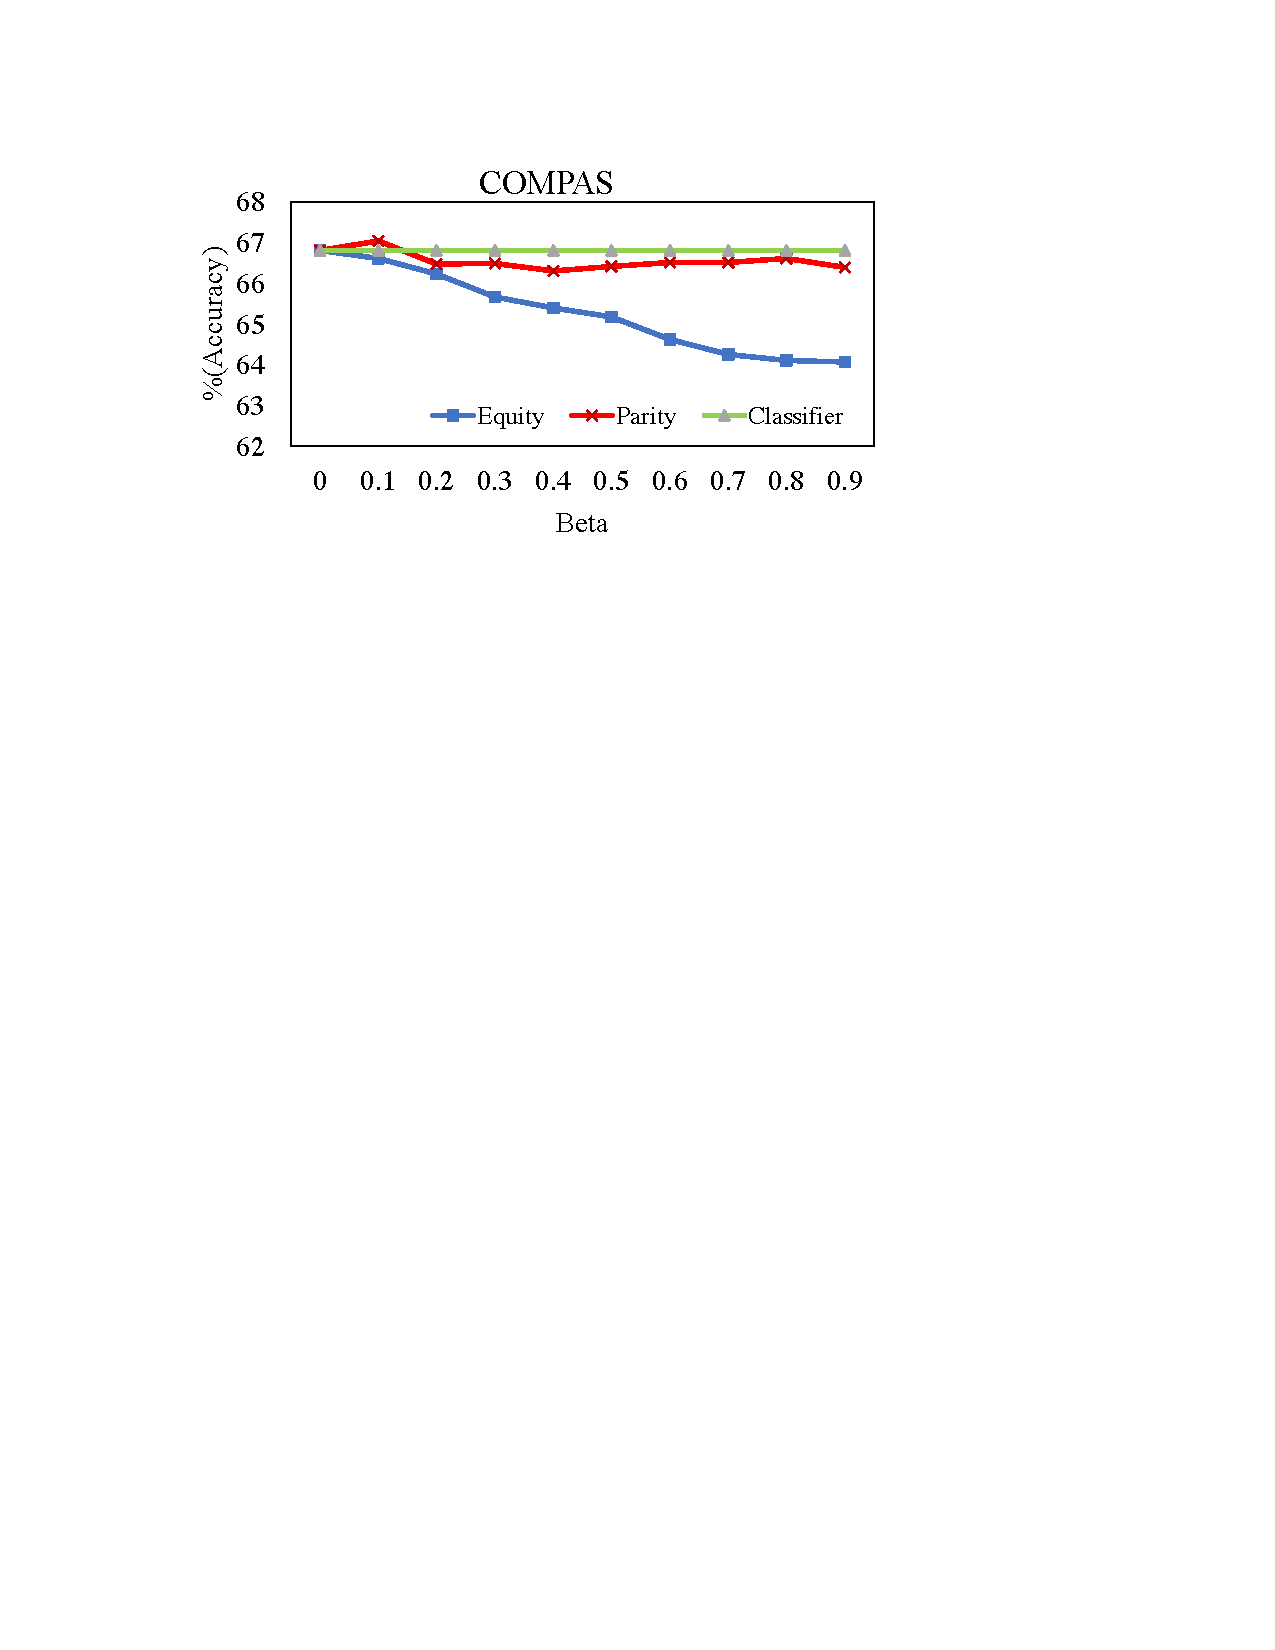
\includegraphics[width=0.45\textwidth,trim=3.0cm 18.9cm 6.5cm 2.5cm,clip=true]{images/compas_times_final.pdf}
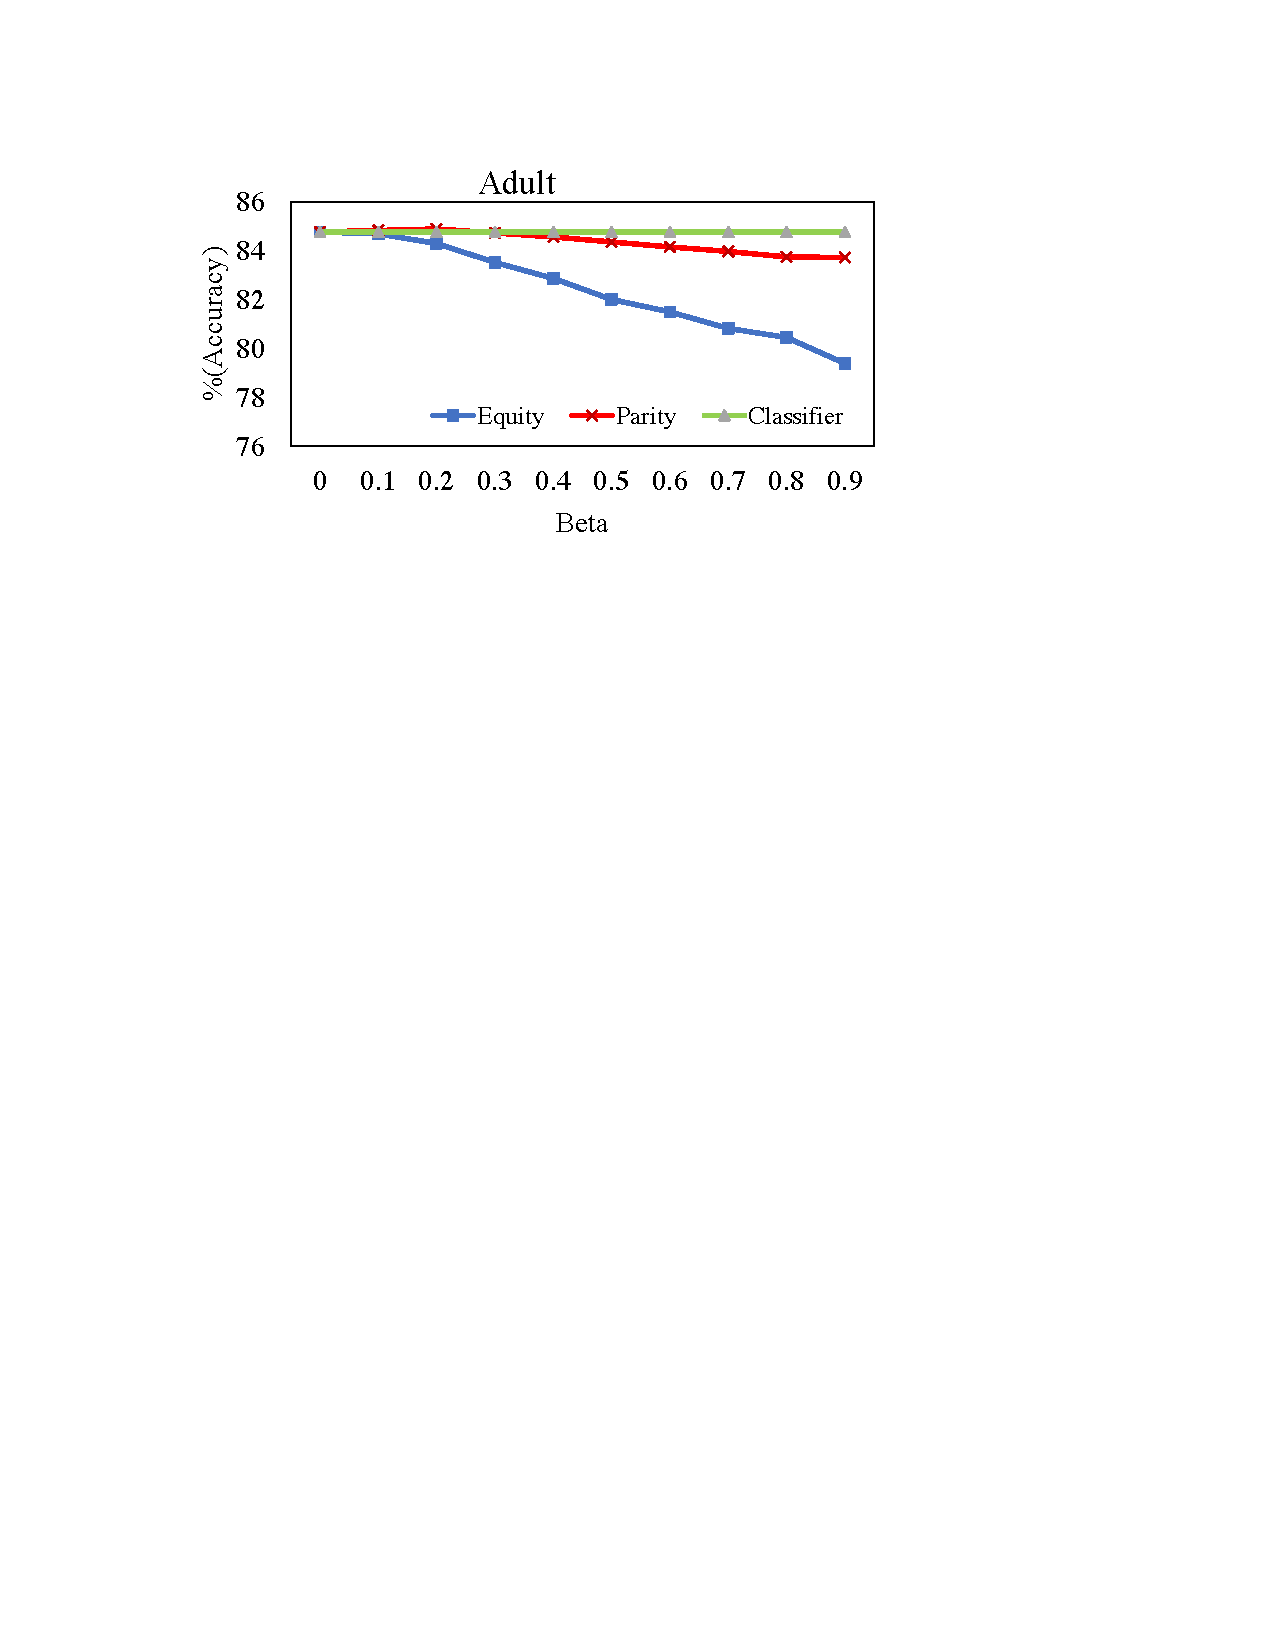
\includegraphics[width=0.45\textwidth,trim=3.0cm 18.9cm 6.5cm 2.5cm,clip=true]{images/adult_times_final.pdf}
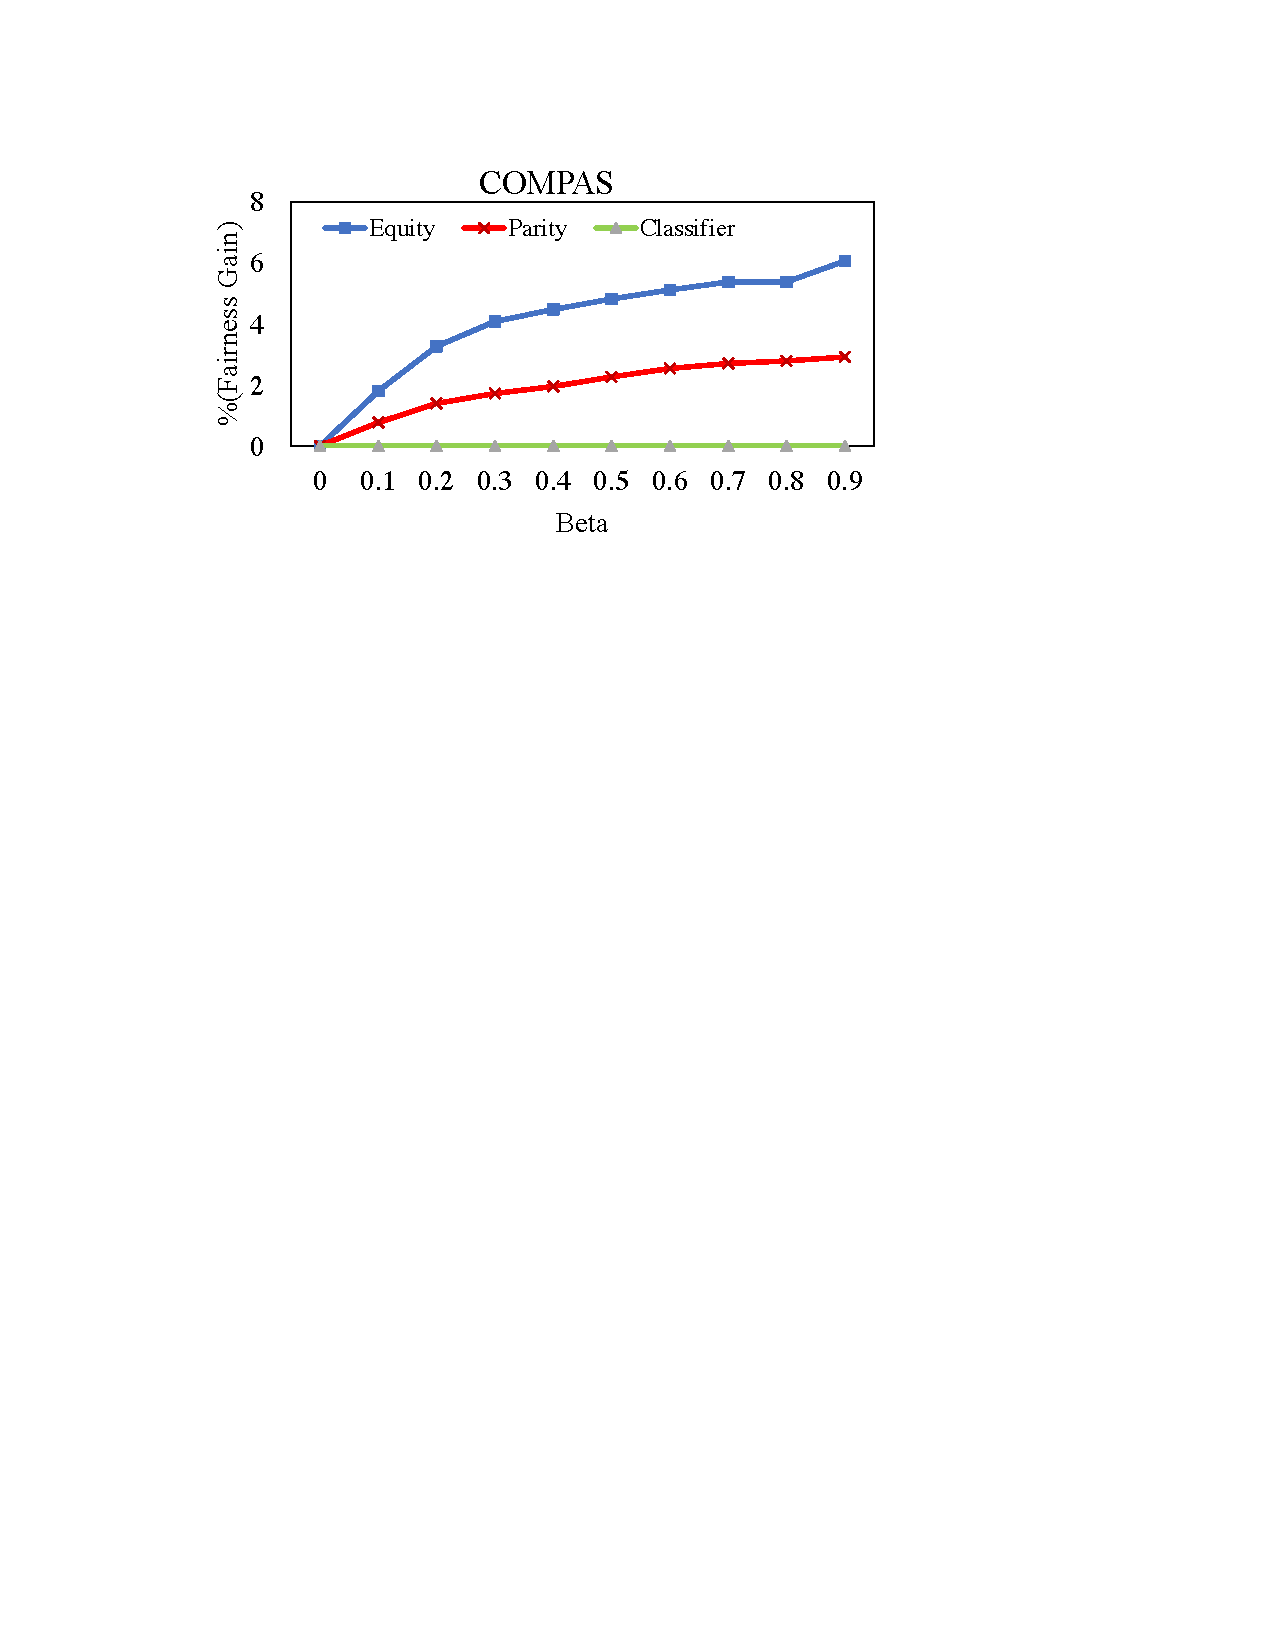
\includegraphics[width=0.45\textwidth,trim=3.0cm 18.9cm 6.5cm 2.5cm,clip=true]{images/compas_fairness_gain.pdf}
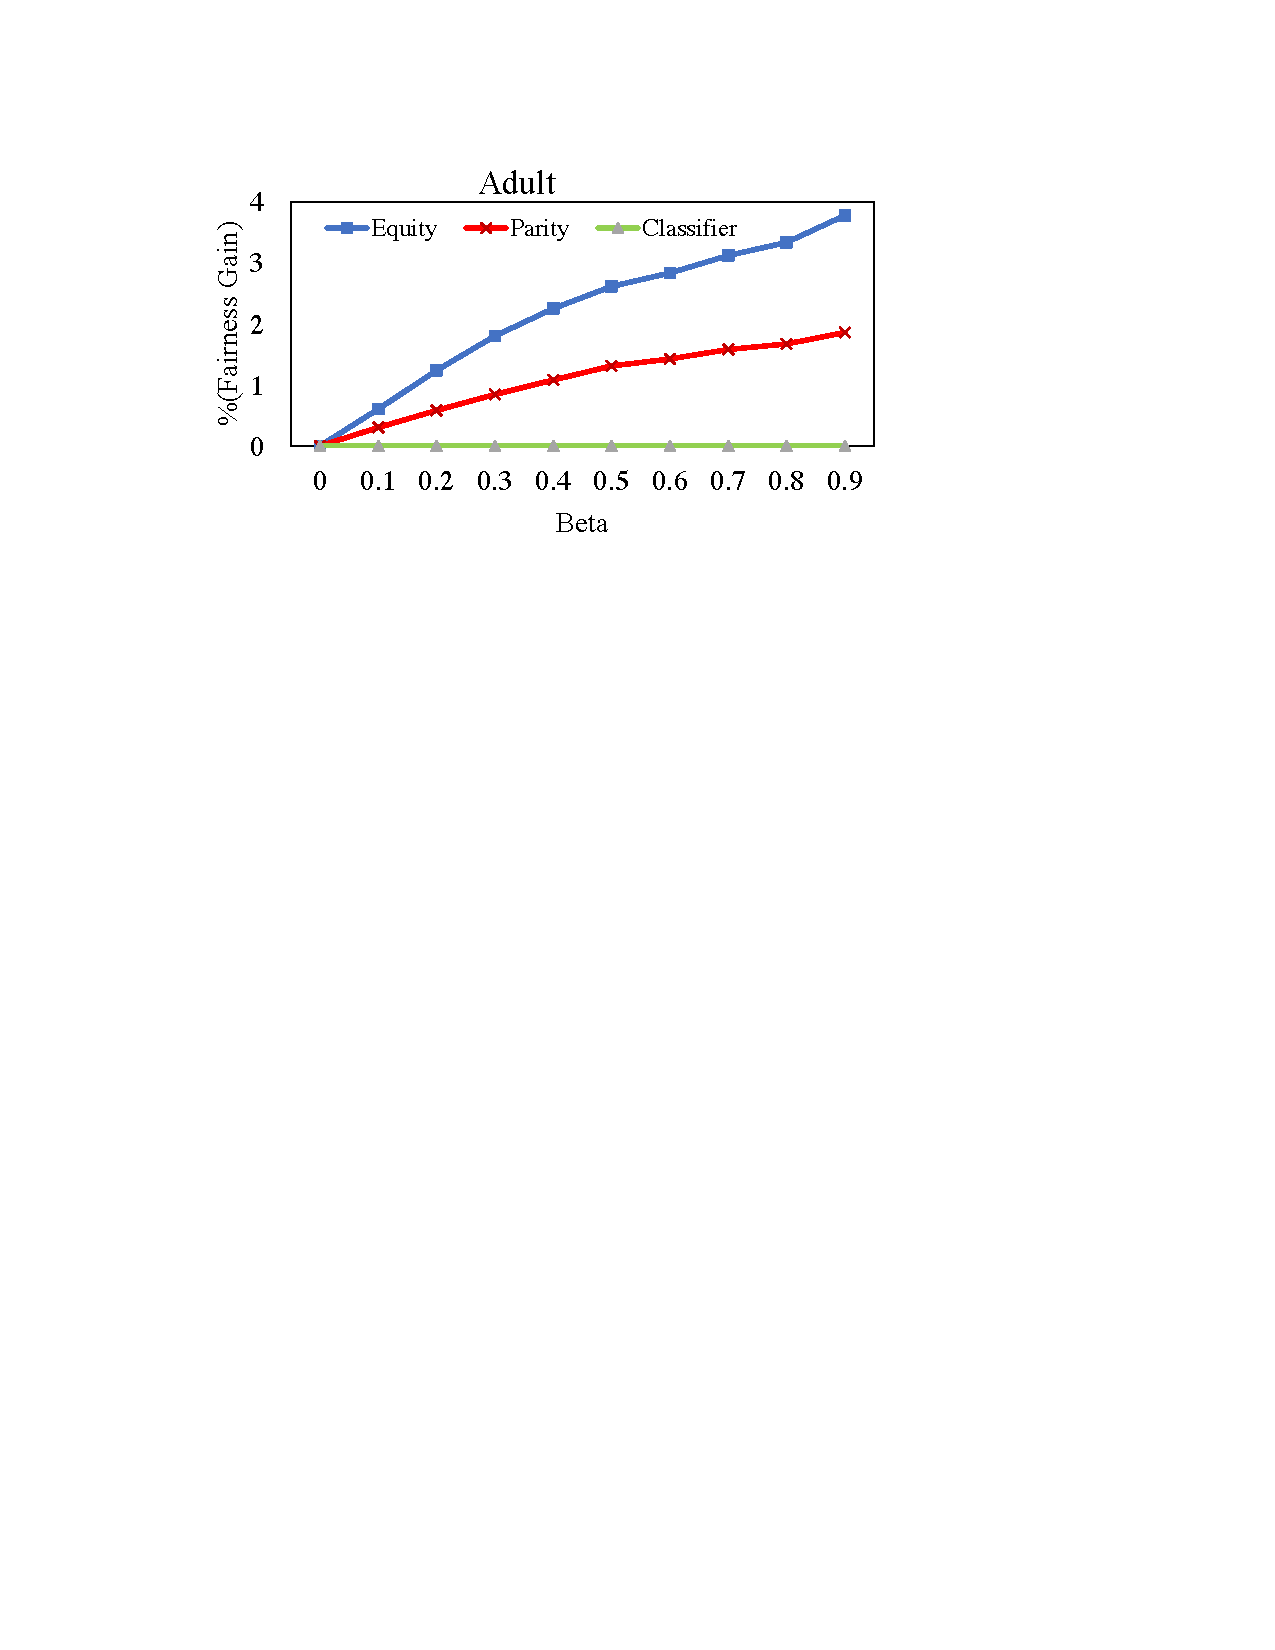
\includegraphics[width=0.45\textwidth,trim=3.0cm 18.9cm 6.5cm 2.5cm,clip=true]{images/adult_fairness_gain.pdf}
\caption{Accuracy and fairness gain results for the COMPAS and Adult datasets over different $\beta$ values. Top plots report the accuracy results, while bottom plots report the fairness gain results. Each point on the plots is the average value of 10 experiments performed on the 10 random splits. Notice that the 10 random split sets are the same across different $\beta$ values. For details of these values along with standard deviation numbers refer to Tables \ref{Adult_acc_gain} and \ref{compas_acc_gain} in the Appendixes section.}
\label{plots1}
\end{figure*}
The model used in these experiments is a two-layer dense network with 256 hidden dimensions. We stopped training the model after seeing no improvement on the validation set for 100 iterations (validation epochs) in all the experiments with a starting learning rate of 0.01 and applied learning rate decay of 0.95. The code is available for reproduction of our experiments.\footnote{\label{projecturl}\url{https://github.com/Ninarehm/Fairness}} We performed the experiments on three different loss functions described below. 
\begin{itemize}
    \item Equity Loss: This loss function is our proposed loss function in Equation~\ref{equity_eq} introduced in the previous section.
    \item Parity Loss: This loss function is mirroring the statistical parity notion of fairness which combines the statistical parity notion with the classification loss as follows: 
    % \begin{align*}
    % min \; F_{parity}(\theta) &= (Pout_1 - Pout_2)^2 \\
    %     &+ (Nout_1 - Nout_2)^2
    % \end{align*}
    \begin{align*}
    &F_\text{parity}(\theta)=\\
    &\sum_{y}\left(\frac{1}{n}\sum_{i=1}^{n}p(\hat{Y_i}=y|A=a) \right. 
    \left.-\frac{1}{n}\sum_{i=1}^{n}p(\hat{Y_i}=y|A=b)\right)^2.
    \end{align*}

    Where $F_\text{parity}$ represents the fairness loss corresponding to the parity notion of fairness. This loss will then be combined with the classification cross-entropy loss as before which will form the whole objective loss as follows:
    \begin{equation}
     \min_\theta \; \beta F_\text{parity}(\theta)+ (1-\beta)L(\theta).
     \label{parity_eq}
    \end{equation}
    \item Classification Loss (Cross-entropy):  This is a loss function containing only the cross-entropy loss with no fairness constraints imposed as follows:
    \begin{equation}
     \min_\theta \; L(\theta).
     \label{classifier_eq}
    \end{equation}
\end{itemize}
In our results, Equity corresponds to a classifier using the equity loss function defined in Equation~\ref{equity_eq}, Parity using the parity loss function defined in Equation~\ref{parity_eq}, and Classifier using the cross-entropy loss only in Equation~\ref{classifier_eq}. We tested these classifiers on two benchmark datasets in fairness, COMPAS and Adult datasets, and reported the performance accuracy and fairness gain as defined below. \\
\begin{mybox}
\begin{definition} [Fairness Gain]
For a given loss function $\ell \in \{\text{Equity},\text{Parity},\text{Classifier}\}$, we define the fairness gain relative to a simple classifier with no fairness constraint for demographic groups $a$ and $b$ on the $D \cup M$ set as:
\begin{align*}
 \text{Fairness Gain}&=\left[|p(Y|A=a)-p(Y|A=b)|\right]_\text{classifier}\\
 & -\left[|p(Y|A=a)-p(Y|A=b)|\right]_\ell.
\end{align*}
In other words, we measure how effective a method was in reducing disparities among demographics compared to a classifier with no fairness constraint. Note how this measure is similar to the statistical parity except considering both the history and future predictive outcome.
\end{definition}
\end{mybox}
For robustness purposes, each of our experiments were performed on 10 random train, validation, and test splits for each of the datasets and the significance of our hypotheses were reported accordingly. The reported results are averages of 10 experiments performed on 10 different random splits. Due to the existing variance in the splits, we found the Mann–Whitney U tests more suitable and reliable in performing experiments. Thus, we reported the significance of the averaged results in terms of $p$-value instead of standard deviation. However, the standard deviations and detailed averaged results are all listed in the appendixes section.  
\begin{tcolorbox}
\begin{hyp} 
The Equity classification objective will achieve the highest gain in fairness, at a slight cost to accuracy. We expect this fairness gain and accuracy degrade to be more noticeable for higher $\beta$ values which controls the importance of fairness gain over classification accuracy.
\end{hyp}
\end{tcolorbox}
\subsection{COMPAS Dataset}
The COMPAS dataset contains information about defendants from Broward County. The labels in our prediction classification task were weather or not a criminal will re-offend within two years. The sensitive attribute in our experiments was gender. Among features in this dataset we used features as listed in Table \ref{compas_features}. We split the dataset into 10 different random 80-10-10 splits for train, test, and validation sets. The averaged accuracy and fairness gain results obtained from applying different losses in our classification task over 10 experiments on different splits with different $\beta$ values on the COMPAS dataset is shown in Figure \ref{plots1}.

From results shown in Figure \ref{plots1}, we can observe that classifier trained on our Equity loss is able to achieve higher fairness gain for all $\beta$ values. We also show the significance of these results in terms of one vs all (Equity vs Parity and Classifier) Mann–Whitney U test in Table \ref{fairness_p} for all the $\beta$ values. Although from the results in Figure \ref{plots1}, one can observe a degrade in performance in terms of test accuracy, the results in Table \ref{accuracy_p} show the insignificance of this degrade for low to mid $\beta$ values in this dataset. However, the degrade gets significant for higher $\beta$ values as expected due to the control of $\beta$ over accuracy-fairness trade-off. Although we reported the results for all the $\beta$ values from 0.1 to extreme of 0.9, we recommend a $\beta$ value around 0.3-0.5 which balances the fairness gain and test accuracy.
% \begin{figure}[!bt]
% \centering
% 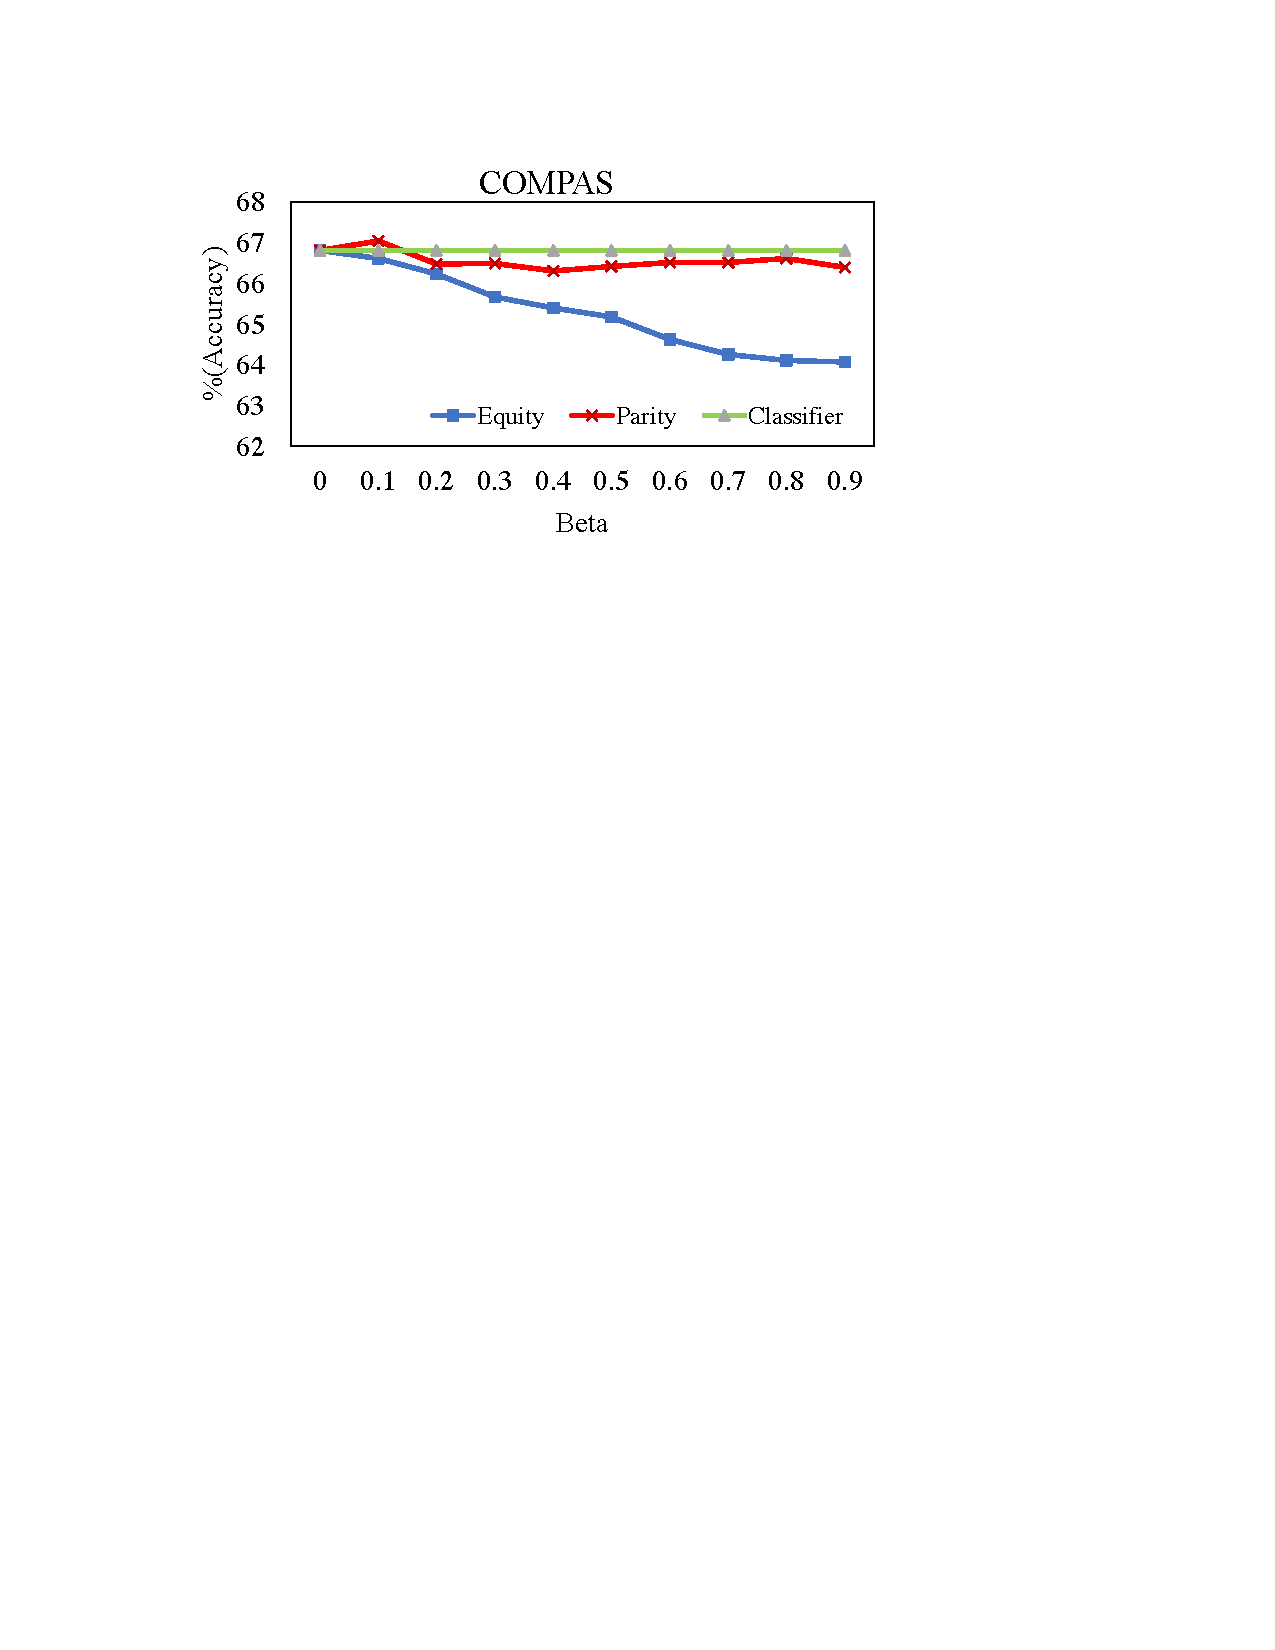
\includegraphics[width=0.23\textwidth,trim=3.5cm 18.9cm 6.7cm 2.7cm,clip=true]{images/compas_times_final.pdf}
% 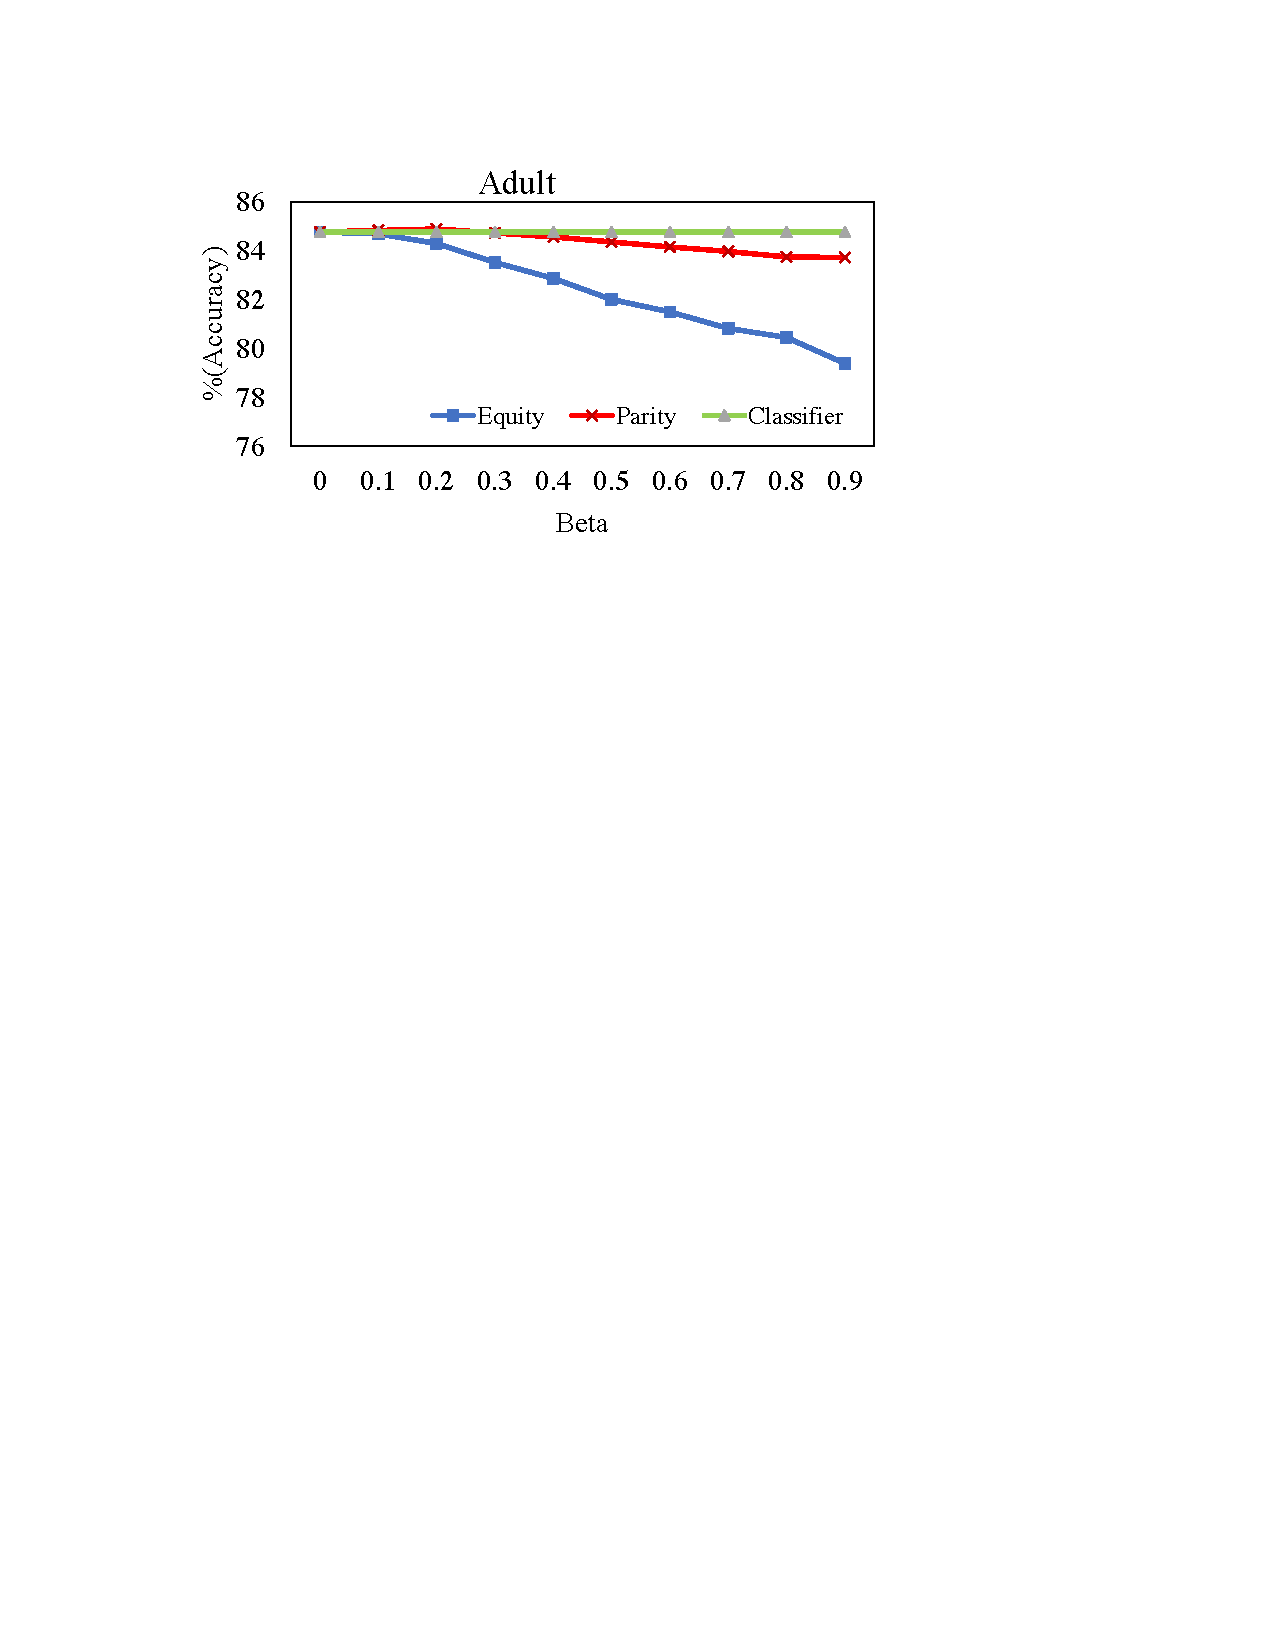
\includegraphics[width=0.23\textwidth,trim=3.5cm 18.9cm 6.7cm 2.7cm,clip=true]{images/adult_times_final.pdf}
% 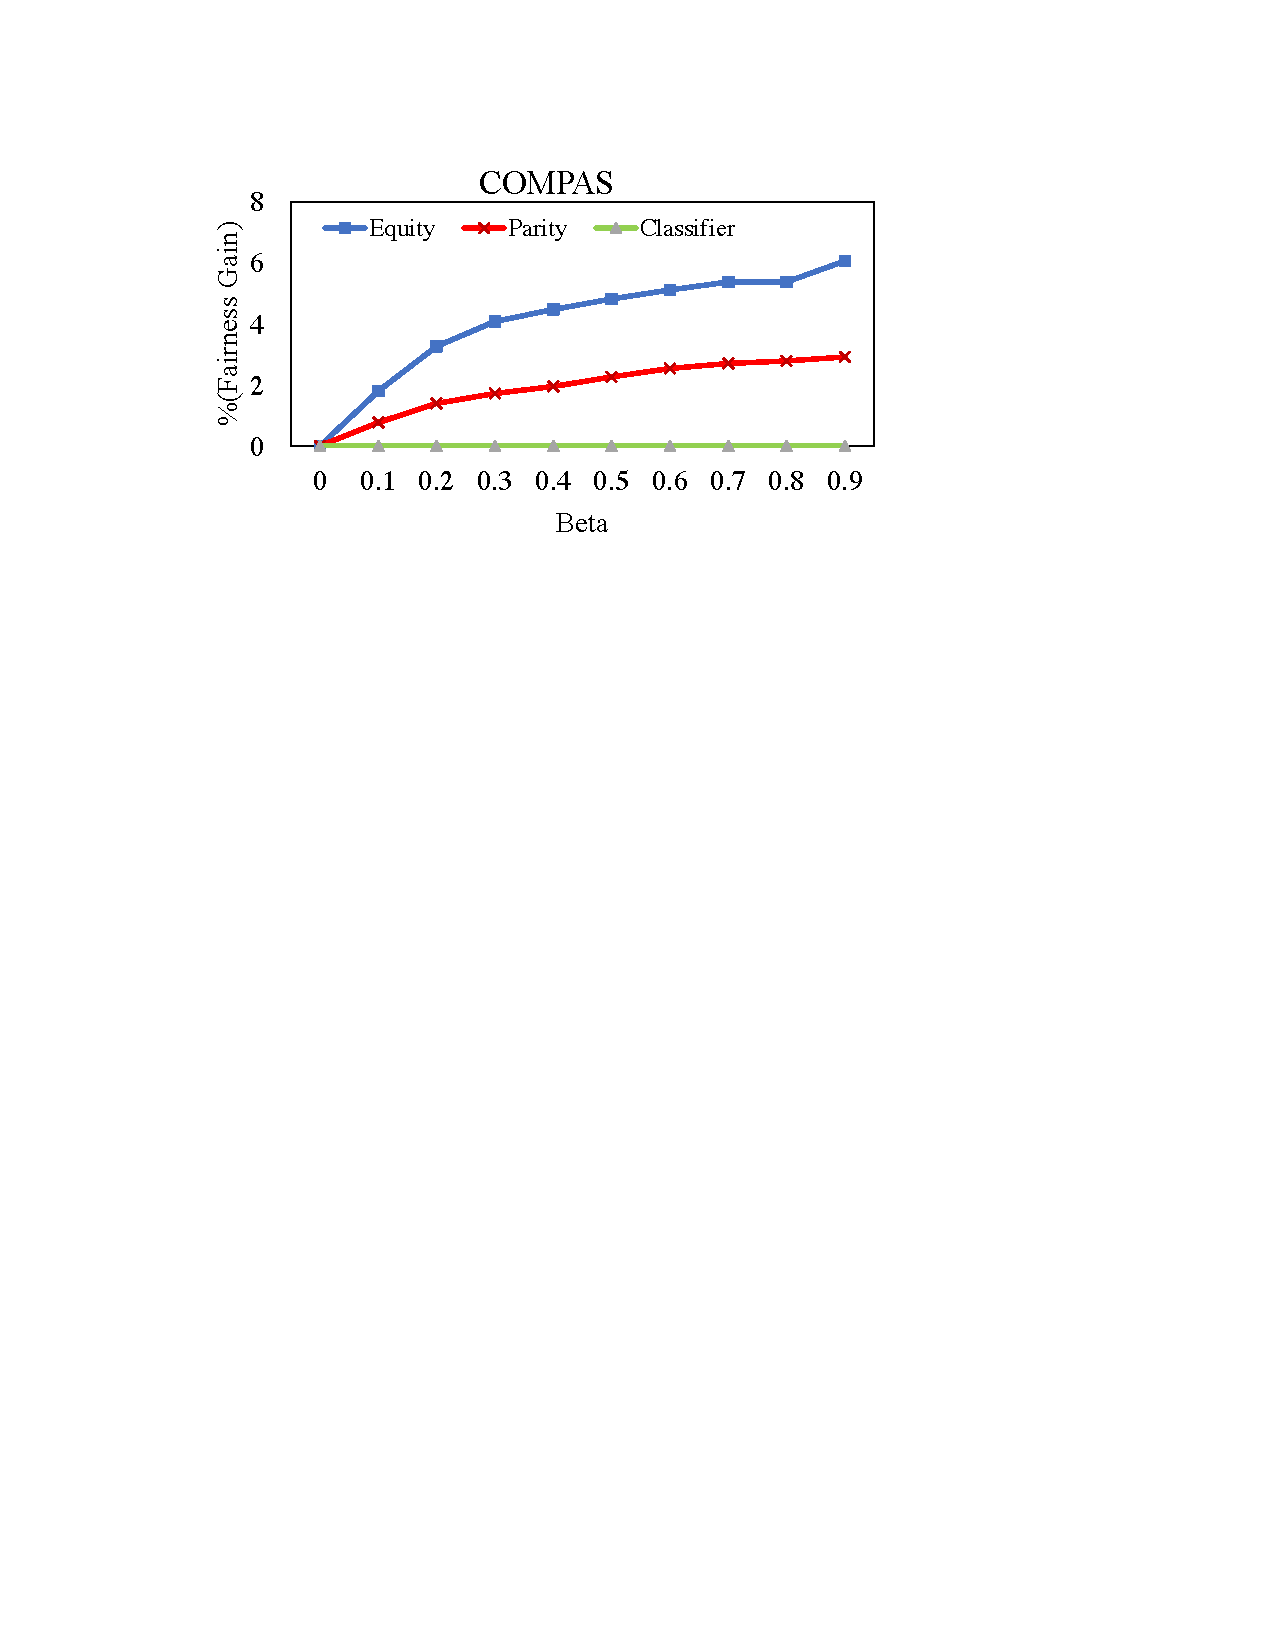
\includegraphics[width=0.23\textwidth,trim=3.5cm 18.9cm 6.7cm 2.7cm,clip=true]{images/compas_fairness_gain.pdf}
% 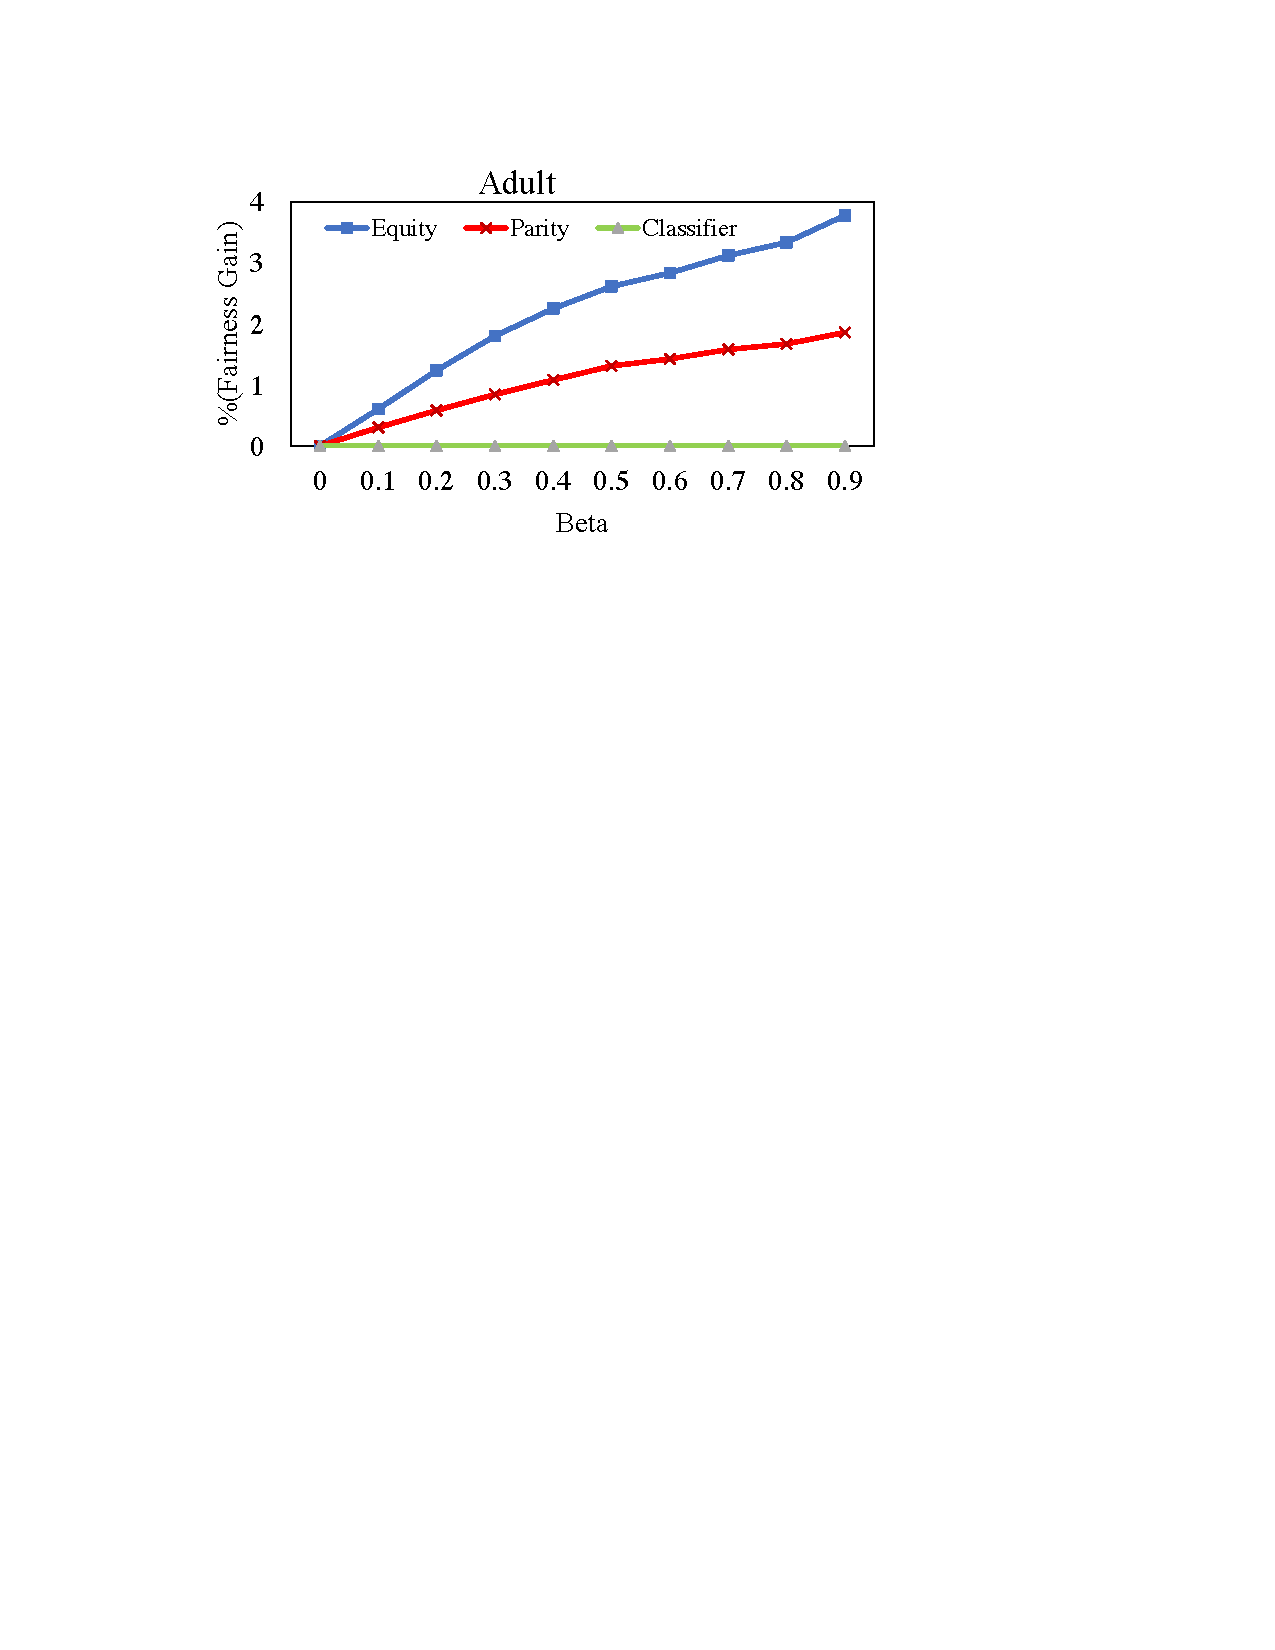
\includegraphics[width=0.23\textwidth,trim=3.5cm 18.9cm 6.7cm 2.7cm,clip=true]{images/adult_fairness_gain.pdf}
% \caption{Accuracy and fairness gain results for the COMPAS and Adult datasets over different $\beta$ values. Top plots report the accuracy results, while bottom plots report the fairness gain results. Each point on the plots is the average value of 10 experiments performed on the 10 random splits. Notice that the 10 random split sets are the same across different $\beta$ values.}
% \label{plots1}
% \end{figure}
% In some papers, the experiments on the COMPAS dataset is performed using the \textit{is\_recid} and \textit{score\_text} features which are highly correlated with the label and that can be interchangeably used as the label. In such results, the classification task achieves more than 95\% accuracy. In our experiments we followed the standard procedure that Propublica took in reporting the results; thus, our results are comparable to propublica's and also many standard fairness papers. However, we have also included results using features that would get us high accuracy values listed in Table \ref{high_compas_features} and reported the results in the Appendixes section of this paper in Table \ref{Compas_results_appendix}.
\subsection{Adult Dataset}
The Adult dataset contains information about individuals with a label corresponding if an individual's income exceeds 50k per year or not. We utilized all the features from the dataset in our classification task for predicting the label. We considered gender as the protected attribute in our classification loss. The data was split into 10 different random 80-10-10 splits for train, test, and validation sets for each set of experiments. The averaged test accuracy and fairness gain results over 10 different splits for each $\beta$ value obtained from applying different losses in our classification task on the Adult dataset is shown in Figure \ref{plots1}.


As shown in Figure \ref{plots1}, we can observe that for all $\beta$ values our definition was able to achieve higher fairness gain. We also show the significance of these results in Table \ref{fairness_p}. Although from the results in Figure \ref{plots1}, one can observe a degrade in performance in terms of test accuracy and that results in Table \ref{accuracy_p} show the significance of this degrade, this degrade is still considered to be a reasonable price for fairness considering the gain in fairness. Especially for mid $\beta$ values in which the degrade can be perceived negligible when considering the gain in fairness. As with the COMPAS dataset, we recommend a $\beta$ value around 0.3-0.5 which balances the fairness gain and test accuracy for this dataset as well. %These results get us a reasonable price for fairness. 
\begin{table}[t]
\begin{tabular}{|p{0.5cm} |c||p{1.07cm}|p{1.15cm}||p{1.07cm}|p{1.15cm}|  }
 \hline
 \multicolumn{2}{|c||}{}&\multicolumn{2}{c||}{COMPAS Dataset}&\multicolumn{2}{c|}{Adult Dataset}\\
 \hline
 \multicolumn{2}{|c||}{}&\multicolumn{2}{c||}{$p$-value}&\multicolumn{2}{c|}{$p$-value}\\
 \hline
Beta& & Parity &Classifier&Parity&Classifier\\
 \hline
0.1&\multirow{8}{*}{\rotatebox[origin=c]{90}{Equity}}   &   0.0003  &3.2e-05  &9.1e-05 &3.2e-05 \\
 0.2&    & 9.1e-05 &3.2e-05 &9.1e-05 & 3.2e-05\\
0.3&&9.1e-05 & 3.2e-05 &9.1e-05&3.2e-05\\
0.4&& 9.1e-05& 3.2e-05 &9.1e-05&3.2e-05\\
0.5&&9.1e-05 & 3.2e-05 &9.1e-05&3.2e-05\\
0.6& & 9.1e-05&3.2e-05  &9.1e-05&3.2e-05\\
0.7& &9.1e-05 &3.2e-05  &9.1e-05&3.2e-05\\
0.8&&0.0001 & 3.2e-05 &9.1e-05&3.2e-05\\
0.9&&9.1e-05 & 3.2e-05&9.1e-05&3.2e-05\\
 \hline
\end{tabular}
\caption{One vs all (Equity loss vs Parity and Classifier losses) Mann–Whitney U test for COMPAS and Adult datasets. The results show the statistical significance of experiments performed for evaluation of fairness gain amongst different losses over different $\beta$ values. The assumed test hypothesis was whether Equity will have greater fairness gain compared to Parity and Classifier losses.}
\label{fairness_p}
\end{table}

\begin{table}[h]
%\centering
\begin{tabular}{ p{2.3cm} p{2.3cm} p{2cm}}
 \toprule
 Features&&\\
 \midrule
 sex&age\_cat&race  \\
 juv\_fel\_count&juv\_misd\_count&juv\_other\_count\\
 priors\_count&c\_charge\_degree&\\[0.5pt]
  \bottomrule
\end{tabular}
\caption{Features used in the experiments from the COMPAS dataset.}
    \label{compas_features}
\end{table}

\subsection{Overall Results Discussion}
As expected in our initial hypothesis, through experimentation and hypothesis testing, we were able to gain knowledge that using the Equity loss in classification will result in gain in fairness. Through Mann–Whitney U significance test we show that this gain is significant for all the $\beta$ values for both of the datasets. With regards to degrade in test accuracy, as expected, larger $\beta$ values resulted in more loss in test accuracy, while more gain in fairness. However, this loss was shown to be non-significant for one of our datasets, the COMPAS dataset, for low to mid $\beta$ values which we recommend using. For the Adult dataset, although the loss was shown to be statistically significant, the test accuracy loss was reasonable considering the price of fairness we get through the gain in fairness. Figure \ref{plots1}, demonstrates the behavior of different losses over different $\beta$ values in terms of test accuracy and fairness gain for the COMPAS and Adult datasets. Tables \ref{fairness_p} and \ref{accuracy_p} indicate the significance of our hypothesis in terms of Equity loss being able to gain highest gain in fairness and also the significance of its degrade in performance in terms of test accuracy over other baselines for the COMPAS and Adult datasets respectively. From the overall results, we suggest use of $\beta$ values between 0.3-0.5 when using our Equity objective as they are shown to be the most effective in terms of gain in fairness and maintaining a reasonable test accuracy. 

\begin{table}[t]
\begin{tabular}{|p{0.5cm} |c||p{1.07cm}|p{1.15cm}||p{1.07cm}|p{1.15cm}|  }
 \hline
 \multicolumn{2}{|c||}{}&\multicolumn{2}{c||}{COMPAS Dataset}&\multicolumn{2}{c|}{Adult Dataset}\\
 \hline
 \multicolumn{2}{|c||}{}&\multicolumn{2}{c||}{$p$-value}&\multicolumn{2}{c|}{$p$-value}\\
 \hline
Beta& & Parity &Classifier&Parity&Classifier\\
 \hline
0.1&\multirow{8}{*}{\rotatebox[origin=c]{90}{Equity}}   &  0.2725   &0.5151  &0.2245 &0.2476 \\
 0.2&   & 0.3383  & 0.1717& 0.0045& 0.0056\\
0.3&&0.1821 &0.0928  &0.0005&0.0003\\
0.4&& 0.1622& 0.0991 &9.1e-05&9.0e-05\\
0.5&& 0.0557& 0.0604 &9.1e-05&9.0e-05\\
0.6& &0.0203 & 0.0377 &9.1e-05&9.1e-05\\
0.7& &0.0187 & 0.0225 &9.1e-05&9.0e-05\\
0.8&&0.0020 & 0.0116 &9.1e-05&9.1e-05\\
0.9&&0.0008 & 0.0069 &9.1e-05&9.1e-05\\
 \hline
\end{tabular}
\caption{One vs all (Equity loss vs Parity and Classifier losses) Mann–Whitney U test for COMPAS and Adult datasets. The results test the statistical significance of experiments performed for evaluation of test accuracy amongst different losses over different $\beta$ values. The test reports the significance of degrade in performance of Equity loss over the other two losses in terms of test accuracy.}
\label{accuracy_p}
\end{table}


